\chapter{Cameras}

\section{Real-world cameras}

\textbf{Idea 1:} Piece of film in front of a scene

\textbf{Idea 2:} Add barrier to block off most of the rays (less blurring)

\textbf{The pinhole camera:} 

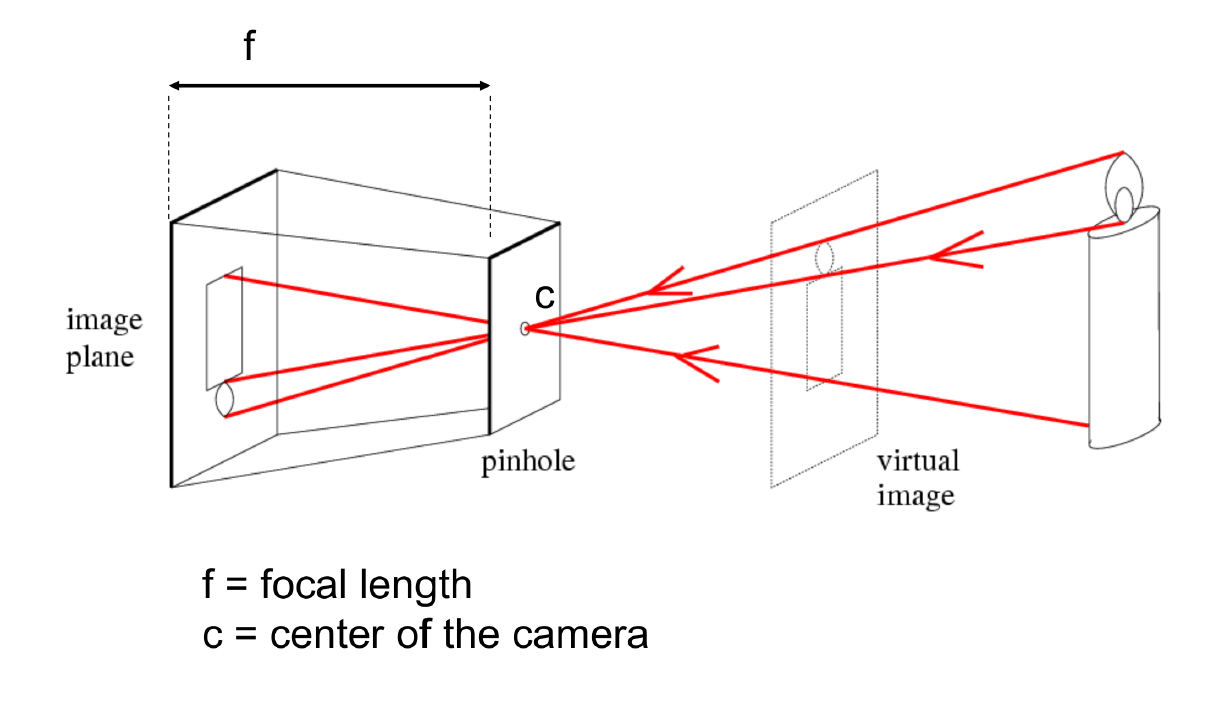
\includegraphics[width=\textwidth]{images/chap7/pinhole}

\textbf{Why lenses?} Pinhole non-zero size, hence object points blurr. Smaller pinhole means \textbf{less blurry}! Can't make arbitrarily small due to physical limitations, i.e., less light goes through, need long exposure, also we have a \textbf{diffraction limit} which means it will ge blurrier at some point.

\textbf{Simple camera design with a single thin lens:}

\textbf{Lens focuses light onto film}: \begin{itemize}
    \item Specific distance at which objects are \textbf{in focus}
    \item Determined by \textbf{focal length}
    \item Points out of focus project to \textbf{circle of confusion}
    \item Larger \textbf{circles of confusion} cause blurr
    \item \textbf{Depth of field} - range in which image appears sharp
\end{itemize}

\textbf{Depth of field and aperture}: Smaller aperture increases range in which object is in focus. Reduces amount of light - need to extend exposure.

\section{Camera models}

Major goal is to extract information of 3D world out of 2D images. Simple case, we consider singe pinhole cameras, i.e., \textbf{monocular vision} which requires \textbf{single view projective geometry}.

\subsection{Pinhole Camera Model}

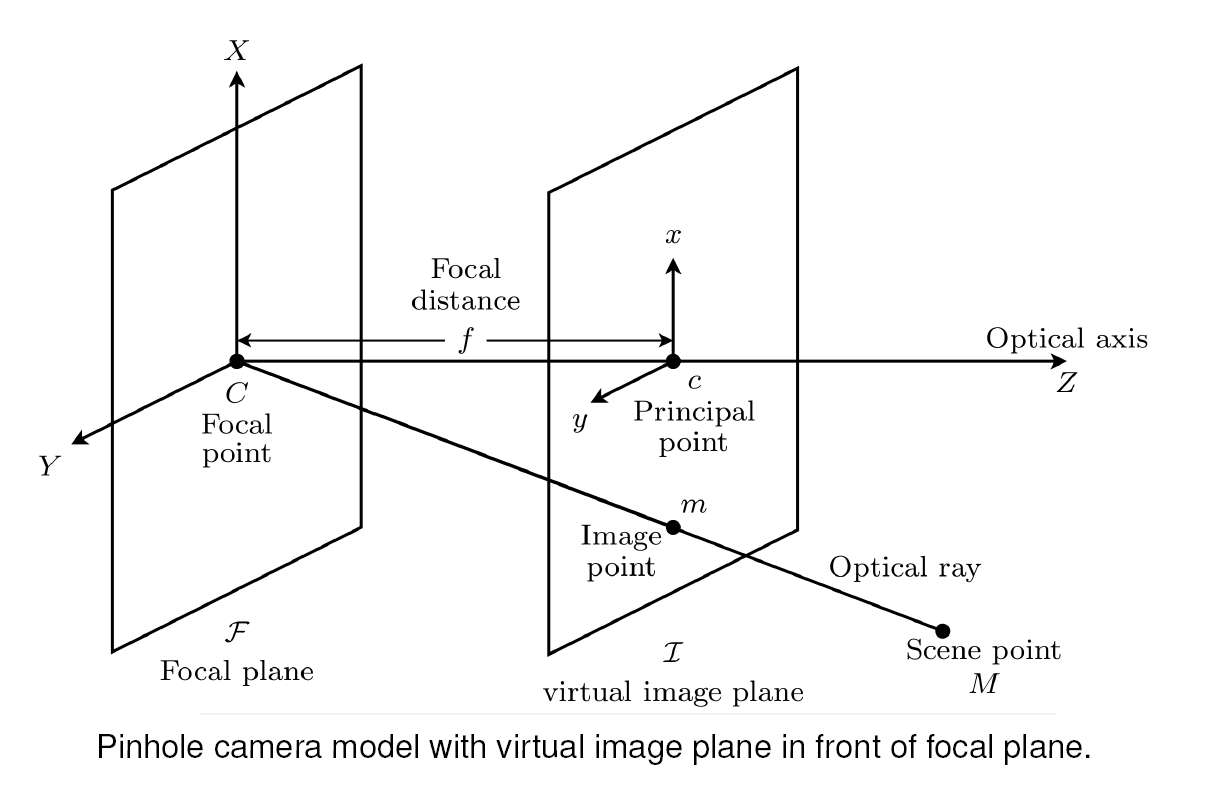
\includegraphics[width=\textwidth]{images/chap7/pinhole_model}

\textbf{Simplified but sufficiently realistic} model of a camera system. Coordinates $(X,Y,Z)$ with origin $C$ map to $m=(x,y)$ with origin $c$.

Notations: \begin{itemize}
    \item $M$, \textbf{scene point}
    \item $C$, \textbf{focal point, optical center}, pinhole location
    \item $m$, \textbf{image point}
    \item $I$, \textbf{image plane}
    \item $F$, \textbf{focal plane}
    \item \textbf{optical axis:} orthogonal to image plane, passes through $C$
    \item \textbf{opical ray:} passes through $M$ and $C$
    \item $f$, \textbf{focal distance}
    \item $c$, \textbf{principal point: intersection} between image plane and optical axis
\end{itemize}

\textbf{Basic geometric relations:} $\frac{x}{X} = \frac{y}{Y} = \frac{f}{Z}$, we see nonuniqueness of projection, since all points on one optical ray with different distances $Z$ are projected to $m = (x,y)$ and we lose depth information.

The previous equation is a nonlinear transformation from 3D to 2D, \textbf{solution?}: \textbf{Lift $m$ to projective space, by adding a coordinate $1$}!

\textbf{Thus}, pinhole projection in homogenous coordinates is projective linear map 
$\mathbb{P}^3 \rightarrow \mathbb{P}^2$: $$\hat{m} = \left[\begin{matrix}
x \\ y \\ 1
\end{matrix}\right] =\left[\begin{matrix}
Zx \\ Zy \\ Z1
\end{matrix}\right] = \left[\begin{matrix}
fX \\ fY \\ Z
\end{matrix}\right] = \underset{P}{\underbrace{\left[\begin{matrix}
f & 0 & 0 & 0 \\ 0 & f & 0 & 0 \\ 0 & 0 & 1 & 0
\end{matrix}\right]}}
\left[\begin{matrix}
X \\ Y \\ Z \\ 1
\end{matrix}\right]$$, with $P$ being the \textbf{Projection Matrix}.

\subsection{Extrinsic Camera Parameters}

Denote position of world coordinates relative to camera coordinates. 3D transformation can be expressed by $4\times 4$ \textbf{matrices}.

\textbf{Translation:} $T = \left[\begin{matrix}
1 & 0 & 0 & t_1 \\ & 0 & 1 & 0 & t_2 \\ 0 & 0 & 1 & t_3 \\ 0 & 0 & 0 & 1
\end{matrix}\right] = \left[ \begin{matrix} I & t \\ 0 & 1 \end{matrix} \right]$,

\textbf{Rotation:} $R = \left[\begin{matrix}
r_{11} & r_{12} & r_{13} & 0 \\ r_{21} & r_{22} & r_{23} & 0 \\ r_{31} & r_{32} & r_{33} & 0 \\ 0 & 0 & 0 & 1
\end{matrix}\right] = \left[\begin{matrix} R & 0 \\ 0 & 1 \end{matrix} \right]$, with $RR^T = R^T R = I_4$, with rotations for

$R_x(\Phi) = \left[\begin{matrix}
1 & 0 & 0 & 0 \\ 0 & \cos \Phi & -\sin \Phi & 0 \\ 0 & \sin \Phi & \cos \Phi & 0 \\ 0 & 0 & 0 & 1
\end{matrix}\right]$, $R_y(\Phi) = \left[\begin{matrix}
\cos \Phi & 0 & -\sin \Phi & 0 \\ 0 & 1 & 0 & 0 \\ \sin \Phi & 0 & \cos \Phi & 0 \\ 0 & 0 & 0 & 1
\end{matrix}\right]$, $R_z(\Phi) = \left[\begin{matrix}
\cos \Phi & -\sin \Phi & 0 & 0 \\ \sin \Phi & \cos \Phi & 0 & 0 \\ 0 & 0 & 1 & 0 \\ 0 & 0 & 0 & 1
\end{matrix}\right]$

\textbf{Rotation and translation} does \textbf{not commute}!

We have \textbf{3 DoF} for translation and \textbf{3 DoF} for rotation (1 angle per axis).

\subsection{Intrinsic Camera Parameters}

Describes transition from image coordinates in world units to pixel coordinates and therefore \textbf{the geometry of the image plane inside the camera}.

\textbf{Frequent properties}: \begin{itemize}
    \item Origin of the image plane can be located in another point than the \textbf{principal point}
    \item Let principal point of new coordinate system be in $(u_0, v_0)$
    \item $(u,v)$ measured in pixel units has e.g., $k,l$ pixels per meter.
\end{itemize}

From these four intrinsic parameters we get the matrix transformation $$\left[\begin{matrix}u \\ v \\ 1 \end{matrix} \right] = \left[\begin{matrix}k & 0 & u_0 \\ 0 & l & v_0 \\ 0 & 0 & 1 \end{matrix} \right]\left[\begin{matrix}x \\ y \\ 1 \end{matrix} \right]$$, which describes transition from projective coordinates to pixel coordinates. $k,l$ scaling and $u_0 , v_0$ for translation.

If the coordinate system is \textbf{skewed}, i.e., v-axis has an angle $\Theta \neq 90°$ to the u-axis we get:
$$\left[\begin{matrix}u \\ v \\ 1 \end{matrix} \right] = \left[\begin{matrix}k & -k \cot\theta & u_0 \\ 0 & l/\sin\theta & v_0 \\ 0 & 0 & 1 \end{matrix} \right]\left[\begin{matrix}x \\ y \\ 1 \end{matrix} \right]$$

In practice skew is assumed to be $0$! Also pixel sizes $k,l$ from manufacturers can generally be trusted.

\textbf{Intrinsic matrix, note on units:} $H$ and $P$ often multiplied to form single \textbf{intrinsic matrix} $K$, \textbf{which transforms from camera coordinates to homogenous pixel coordinates}:
$$K = \underset{H}{\underbrace{\left[\begin{matrix}k & -k \cot\theta & u_0 \\ 0 & l/\sin\theta & v_0 \\ 0 & 0 & 1 \end{matrix} \right]\left[\begin{matrix}x \\ y \\ 1 \end{matrix} \right]}} \underset{P}{\underbrace{\left[\begin{matrix} f & 0 & 0 & 0 \\ 0 & f & 0 & 0 \\ 0 & 0 & 1 & 0\end{matrix}\right]}} = \left[\begin{matrix}kf & -kf \cot\theta & u_0  & 0\\ 0 & lf/\sin\theta & v_0 & 0 \\ 0 & 0 & 1 & 0 \end{matrix} \right]$$

\textbf{Focal length $f$} usually given in physical unit (meters) and as $k,l$ (pixels per meter).

\textbf{Note:} Only depends on \textbf{products} $\alpha = kf , \beta = lf$, \textbf{magnification} of the system measured in pixels.

\subsection{Complete Pinhole Camera Model}

Combination of extrinsic and intrinsic parameters to map from \textbf{homogenous world coordinates} to \textbf{homogenous pixel coordinates} is given by:

$$\left[\begin{matrix}
Zu \\ Zv \\ Z
\end{matrix}\right] = \underset{=:\Pi}{\underbrace{KTR}} \left[\begin{matrix}
X_W \\ Y_W \\ Z_W \\ 1
\end{matrix}\right]$$

$K, 3\times 4$ intrinsic matrix, $R, 4\times 4$ rotation matrix, $T, 4\times 4$ translation matrix. Te \textbf{perspective projection matrix} complete describes the camera model with \textbf{11 DoF}, due to arbitrary scale factors from homgenous coordinates: $\Pi = \left[\begin{matrix}
    \pi_{11} & \pi_{12} & \pi_{13} & \pi_{14} \\
    \pi_{21} & \pi_{22} & \pi_{23} & \pi_{24} \\
    \pi_{31} & \pi_{32} & \pi_{33} & \pi_{34}
\end{matrix}\right]$. 

\textbf{Simplification} with the \textbf{affine} camera model is given by $\Pi_{affine} = \left[\begin{matrix}
    \pi_{11} & \pi_{12} & \pi_{13} & \pi_{14} \\
    \pi_{21} & \pi_{22} & \pi_{23} & \pi_{24} \\
    0&0&0&Z_{const}
\end{matrix}\right]$, if the scene points approx. have same distance $Z_{const}$ and has \textbf{6 DoF} since the 8 parameters are not independent. The mapping \textbf{is completely linear}.

\section{Geometry of perspective projection}

\textbf{Properties:}\begin{itemize}
    \item \textbf{Many-to-one}: Points along ray map to same point
    \item \textbf{Points map to points}: Projection on focal plane is undefined
    \item \textbf{Lines map to lines:} Lines through focal point (visual rays) project to a point.
    \item \textbf{Convex sets in 3D map to convex sets in 2D}
\end{itemize}

\subsection{Vanishing points}

Lines parallel in world coordinates vanish in a single point.

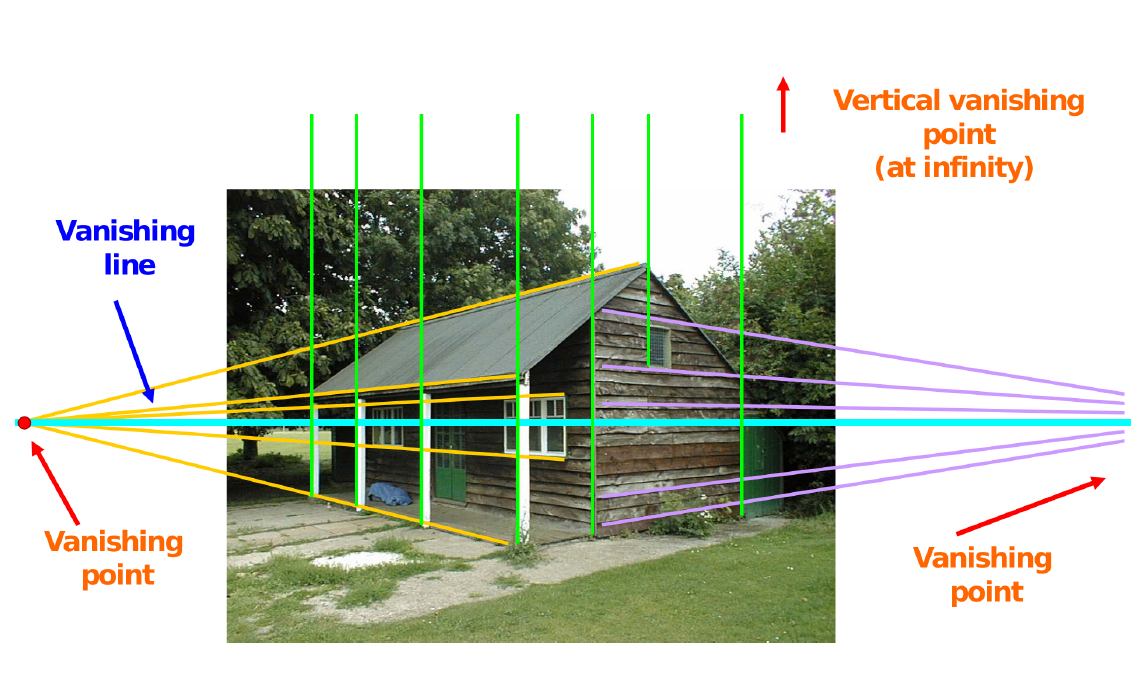
\includegraphics[width=\textwidth]{images/chap7/vanishing_points}

\textbf{Vanishing lines} are what lines parallel to a plane converge to (ground plane -> horizon).

\textbf{Computation 1:} Given line in world coordinates $Mt = \rectmat{x_0 \\ y_0 \\ z_0} + \rectmat{\alpha \\ 0 \\ 1}t$ calculate projection into homogeneous coordinates:

$$PM_t = \rectmat{f&0&0&0 \\ 0&f&0&0 \\ 0&0&1&0} \rectmat{x_0 + \alpha t \\ y_0 \\ z_0 + t \\ 1} = \rectmat{f(x_0 + \alpha t) \\ fy_0 \\ z_0 + 1} \hat{=} \rectmat{\frac{f(x_0 + \alpha t)}{z_0 + t} \\ \frac{fy_0}{z_0 + t} \\ 1}$$. To calculate the vanishing point we have to calculate the limit for $t \rightarrow \infty$:

$$\lim\limits_{t\rightarrow \infty} mt = \lim\limits_{t\rightarrow \infty}\rectmat{\frac{f(x_0 + \alpha t)}{z_0 + t} \\ \frac{fy_0}{z_0 + t} \\ 1} = \lim\limits_{t\rightarrow \infty}\rectmat{\frac{f\alpha t}{z_0 + t} \\ 0 \\ 1} = \lim\limits_{t\rightarrow \infty}\rectmat{\frac{f\alpha t}{t(\frac{z_0}{t} + 1)} \\ 0 \\ 1} = \rectmat{f\alpha \\ 0 \\ 1}$$

\textbf{Computation 2:} Compute the horizon, the set of all vanishing points of lines parallel to the ground plane. A line on the ground plane can be written as a line where the the y-coordinate is not change by parameter $t$:

$Mt = \rectmat{x_0 \\ y_0 \\ z_0} + \rectmat{\alpha \\ 0 \\ \beta}t$, going through the same process as before, i.e. multiplying the matrices we get $$m_t = \rectmat{f&0&0&0 \\ 0&f&0&0 \\ 0&0&1&0} \rectmat{x_0 + \alpha t \\ y_0 \\ z_0 + \beta t \\ 1}  \hat{=} \rectmat{\frac{f(x_0 + \alpha t)}{z_0 + \beta t} \\ \frac{fy_0}{z_0 + \beta t} \\ 1}$$

calculating the limit of $t\rightarrow \infty$, we get for the horizon:

$$\lim\limits_{t\rightarrow \infty} mt = \lim\limits_{t\rightarrow \infty}\rectmat{\frac{f(x_0 + \alpha t)}{z_0 + \beta t} \\ \frac{fy_0}{z_0 + \beta t} \\ 1} = \lim\limits_{t\rightarrow \infty}\rectmat{\frac{f\alpha t}{z_0 + \beta t} \\ 0 \\ 1} = \lim\limits_{t\rightarrow \infty}\rectmat{\frac{f\alpha t}{t(\frac{z_0}{t} + \beta)} \\ 0 \\ 1} = \rectmat{\frac{f\alpha}{\beta} \\ 0 \\ 1}$$

\textbf{Computation 3:} The camera moves up $C$ units in world coordinates. By the last result we have mathematical prove that the horizon stays \textbf{stationary}!

\textbf{Computation 4:}  Optical center fixed, camera rotated 15 degrees around X-axis. Recalculating all possible directions: $$d'(\alpha, \beta) = R_X(\Phi)d(\alpha,\beta) = \rectmat{1 & 0 & 0 & 0 \\ 0 & \cos \Phi & -\sin \Phi & 0 \\ 0 & \sin \Phi & \cos \Phi & 0 \\ 0 & 0 & 0 & 1} \rectmat{\alpha \\ 0 \\ \beta \\ 1} = \rectmat{\alpha \\ -\beta \sin\Phi \\ \beta \cos \Phi \\ 1}$$, this is only the new direction vector, we need to calculate the horizon using this direction vector, as we've done before, going through all calculations we end up at the horizon $$\rectmat{\frac{f\alpha}{\beta\cos\Phi} \\ -\frac{f\sin\Phi}{\cos\Phi} \\ 1} = \rectmat{\frac{f\alpha}{\beta\cos\Phi} \\ -f \tan \Phi \\ 1}$$. In this example the horizon \textbf{moves up} $-\tan(-15°) * f) = 0.2679 * f$ pixels.

\subsection{Perspective distortion}

\textbf{Center of mass in 3D does not map to center of mass in 2D}, i.e., for spheres we get ellipses if they are not the center of the image.

\textbf{Are homographies given when} \begin{itemize}
    \item Translating cameras: Not always, objects can get in front of the scene
    \item Capturing images of a plane: Yes
    \item Rotation: Yes
\end{itemize}

\textbf{Why are planes homographies?} We can assume \textbf{WCS} is chosen, s.t. the plane is parametrized in world coordinates with $[p \ q \ 0 \ 1]^T$. Applying $PRT$ on this point we get a homography.

\textbf{Punchline 1:} Planar surfaces in 3D, reduces projection to a 2D to 2D transformation.

\textbf{Punchline 2:} Transformation is invertible!

\textbf{Why is rotation of the camera still homography?} Let $\rectmat{u \\ v \\ 1} \hat{=} K \rectmat{X \\ Y \\ Z}$ be the primary projection. When rotated we can write $\rectmat{u' \\ v '\\ 1} \hat{=} KR \rectmat{X \\ Y \\ Z} = KRK^{-1}K \rectmat{X \\ Y \\ Z} \hat{=}  KRK^{-1} \rectmat{u \\ v \\ 1}$

$KRK^{-1}$ is the homography between images (called "conjugate relation").

\section{Pinhole camera calibration}

\textbf{What needs to be done?} \begin{itemize}
    \item Determine the \textbf{5 intrinsic} and \textbf{6 extrinsic} parameters
    \item Many algos proposed
    \item \textbf{Basic idea:} Investigate image of \textbf{known} size and shape
    \item Identified point corresponds to 2 constraints
    \item For 11 parameters we need 6 correspondences
    \item Considering more points, makes estimation less sensitive w.r.t. errors
\end{itemize}

\subsection{Basic equations}

\textbf{Input:} We have $k$ correspondences (for which we know the world to image correspondences)

\textbf{Output:} Perspective projection matrix $\Pi = \left[\begin{matrix}
    \pi_{11} & \pi_{12} & \pi_{13} & \pi_{14} \\
    \pi_{21} & \pi_{22} & \pi_{23} & \pi_{24} \\
    \pi_{31} & \pi_{32} & \pi_{33} & \pi_{34}
\end{matrix}\right]$, with $$\widehat{\rectmat{u^i \\ v^i}} = \rectmat{u^i \\ v^i \\ 1} \hat{=} \rectmat{Z^i u^i \\ Z^i v^i \\ Z^i} = \rectmat{\pi_{11} & \pi_{12} & \pi_{13} & \pi_{14} \\
    \pi_{21} & \pi_{22} & \pi_{23} & \pi_{24} \\
    \pi_{31} & \pi_{32} & \pi_{33} & \pi_{34}} \rectmat{X^i_w \\ Y^i_w \\ Z^i_w \\ 1}$$

\textbf{Problem}: We do not know $Z$ since we lost \textbf{DEPTH} information during projection.

As for the homography estimation, we get two equations per correspondence: \begin{align*}(\pi_{31}X^i_w + \pi_{32}Y^i_w + \pi_{33}Z^i_w + \pi_{34}) u^i & = \pi_{11}X^i_w + \pi_{12}Y^i_w + \pi_{13}Z^i_w + \pi_{14}\\
    (\pi_{31}X^i_w + \pi_{32}Y^i_w + \pi_{33}Z^i_w + \pi_{34}) v^i & = \pi_{21}X^i_w + \pi_{22}Y^i_w + \pi_{23}Z^i_w + \pi_{24}
\end{align*} with the following \textbf{(homogeneous) linear system}: 

$$\rectmat{& & & & & & \vdots & & & & & \\
-X^i_W & -Y^i_W & -Z^i_W & -1 & 0 & 0 & 0 & 0 & u^i X^i_W & u^i Y^i_W & u^i Z^i_W & u^i\\
0 & 0 & 0 & 0 & -X^i_W & -Y^i_W & -Z^i_W & -1 & v^i X^i_W & v^i Y^i_W & v^i Z^i_W & v^i\\
& & & & & & \vdots & & & & &}
\rectmat{\pi_{11} \\\pi_{12} \\ \pi_{13} \\ \pi_{14} \\ \pi_{21} \\ \pi_{22} \\ \pi_{23} \\ \pi_{24} \\ \pi_{31} \\ \pi_{32} \\ \pi_{33} \\ \pi_{34}} = 0$$,

we again want to solve $Ax = 0$ using least squares: $$\mathrm{argmin} || Ax ||^2$$, this can be solved using the \textbf{SVD}!

\subsection{Solving homogeneous system using SVD}

\textbf{Formally,} $A = U\Sigma V^T$, thus $$||Ax||^2 = (Ax,Ax) = x^T(A^T A) x = (V^Tx)^T \Sigma^2 V^T x$$

\textbf{Algorithm:} \underline{Direct linear transformation}

\begin{itemize}
    \item For $k$ correspondences, compute $2k \times 12$ matrix $A$ (set of basic equations)
    \item Compute the SVD
    \item The last column of $V$ is the entries of $\Pi$ since it corresponds to the smalles singular value!
\end{itemize}

\subsection{World to image correspondences}

For this we need a \textbf{Calibration object} with known geometry. Can be previously selected and placed, can also be already in the scene but known.

\textbf{Need to locate correspondences with subpixel precision for exact calibration!}

\subsection{Degenerate Configurations}

Choice of correspondences, s.t. there is no unique solution. Even close to degenerate choices lead to unstable results. Select correspondences in general positions.

\textbf{Important degenerate} configuration is if all points lie on one plane. 

\subsection{Constraints due to knowledge of camera}

\textbf{Useful theorem:} $\Pi , 3\times 4$ projection matrix, $a_i^T$ rows of $A$ which is formed of the left-three-columns of $\Pi$: \begin{itemize}
    \item $\Pi$ is a projection matrix iff $\det(A) \neq 0$
    \item $\Pi$ is zero-skew iff additionally $(a_1 \times a_3) \cdot (a_2 \times a_3) = 0$
    \item $\Pi$ has unit aspect ratio (square pixels) iff $(a_1 \times a_3) \cdot (a_1 \times a_3) = (a_2 \times a_3) \cdot (a_2 \times a_3)$
\end{itemize}